%% abtex2-modelo-projeto-pesquisa.tex, v-1 PFC 1 2016
%% Copyright 2012-2015 by abnTeX2 group at http://www.abntex.net.br/ 
%%
%% This work consists of the files abntex2-modelo-projeto-pesquisa.tex
%% and abntex2-modelo-references.bib
%%

% ------------------------------------------------------------------------
% ------------------------------------------------------------------------
% abnTeX2: Modelo de Projeto de pesquisa em conformidade com 
% ABNT NBR 15287:2011 Informação e documentação - Projeto de pesquisa -
% Apresentação 
% ------------------------------------------------------------------------ 
% ------------------------------------------------------------------------

\documentclass[
	% -- opções da classe memoir --
	12pt,				% tamanho da fonte
	openright,			% capítulos começam em pág ímpar (insere página vazia caso preciso)
	oneside,
    %twoside,			% para impressão em verso e anverso. Oposto a oneside
	a4paper,			% tamanho do papel. 
	% -- opções da classe abntex2 --
	%chapter=TITLE,		% títulos de capítulos convertidos em letras maiúsculas
	%section=TITLE,		% títulos de seções convertidos em letras maiúsculas
	%subsection=TITLE,	% títulos de subseções convertidos em letras maiúsculas
	%subsubsection=TITLE,% títulos de subsubseções convertidos em letras maiúsculas
	% -- opções do pacote babel --
	english,			% idioma adicional para hifenização
	french,				% idioma adicional para hifenização
	spanish,			% idioma adicional para hifenização
	brazil,				% o último idioma é o principal do documento
	]{abntex2}

% ---
% PACOTES
% ---

% ---
% Pacotes fundamentais 
% ---
\usepackage{lmodern}			% Usa a fonte Latin Modern
\usepackage[T1]{fontenc}		% Selecao de codigos de fonte.
\usepackage[utf8]{inputenc}		% Codificacao do documento (conversão automática dos acentos)
\usepackage{indentfirst}		% Indenta o primeiro parágrafo de cada seção.
\usepackage{color}				% Controle das cores
\usepackage{graphicx}			% Inclusão de gráficos
\usepackage{microtype} 			% para melhorias de justificação
% ---

% ---
% Pacotes adicionais, usados apenas no âmbito do Modelo Canônico do abnteX2
% ---
\usepackage{lipsum}				% para geração de dummy text
% ---

% ---
% Pacotes de citações
% ---
\usepackage[brazilian,hyperpageref]{backref}	 % Paginas com as citações na bibl
\usepackage[alf]{abntex2cite}	% Citações padrão ABNT

% --- 
% CONFIGURAÇÕES DE PACOTES
% --- 

% ---
% Configurações do pacote backref
% Usado sem a opção hyperpageref de backref
\renewcommand{\backrefpagesname}{Citado na(s) página(s):~}
% Texto padrão antes do número das páginas
\renewcommand{\backref}{}
% Define os textos da citação
\renewcommand*{\backrefalt}[4]{
	\ifcase #1 %
		Nenhuma citação no texto.%
	\or
		Citado na página #2.%
	\else
		Citado #1 vezes nas páginas #2.%
	\fi}%
% ---

% ---
% Informações de dados para CAPA e FOLHA DE ROSTO
% ---
\titulo{Título da Pesquisa e/ou Trabalho}
\autor{Aluno do Curso de Ciências da Computação}
\local{Jataí-GO}
\data{2016}
\tipotrabalho{Projeto de Pesquisa (Graduação)}
% O preambulo deve conter o tipo do trabalho, o objetivo, 
% o nome da instituição e a área de concentração 
\preambulo{Projeto de Pesquisa apresentado ao curso de Bacharelado em Ciências da Computação, como requisito para obtenção do grau final na disciplina de Projeto Final de Curso 1. }

\orientador {Prof. Dr. Orientador do Aluno}

\instituicao{
  Universidade Federal de Goiás - Regional Jataí}


% ---

% ---
% Configurações de aparência do PDF final

% alterando o aspecto da cor azul
\definecolor{blue}{RGB}{41,5,195}

% informações do PDF
\makeatletter
\hypersetup{
     	%pagebackref=true,
		pdftitle={\@title}, 
		pdfauthor={\@author},
    	pdfsubject={\imprimirpreambulo},
	    pdfcreator={LaTeX with abnTeX2},
		pdfkeywords={abnt}{latex}{abntex}{abntex2}{projeto de pesquisa}, 
		colorlinks=true,       		% false: boxed links; true: colored links
    	linkcolor=blue,          	% color of internal links
    	citecolor=blue,        		% color of links to bibliography
    	filecolor=magenta,      		% color of file links
		urlcolor=blue,
		bookmarksdepth=4
}
\makeatother
% --- 

% --- 
% Espaçamentos entre linhas e parágrafos 
% --- 

% O tamanho do parágrafo é dado por:
\setlength{\parindent}{1.3cm}

% Controle do espaçamento entre um parágrafo e outro:
\setlength{\parskip}{0.2cm}  % tente também \onelineskip

% ---
% compila o indice
% ---
\makeindex
% ---

% ----
% Início do documento
% ----
\begin{document}

% Seleciona o idioma do documento (conforme pacotes do babel)
%\selectlanguage{english}
\selectlanguage{brazil}

% Retira espaço extra obsoleto entre as frases.
\frenchspacing 

% ----------------------------------------------------------
% ELEMENTOS PRÉ-TEXTUAIS
% ----------------------------------------------------------
% \pretextual

% ---
% Capa
% ---
\imprimircapa
% ---

% ---
% Folha de rosto
% ---
\imprimirfolhaderosto
% ---

% ---
% NOTA DA ABNT NBR 15287:2011, p. 4:
%  ``Se exigido pela entidade, apresentar os dados curriculares do autor em
%     folha ou página distinta após a folha de rosto.''
% ---

% ---
% inserir lista de ilustrações
% ---
\pdfbookmark[0]{\listfigurename}{lof}
\listoffigures*
\cleardoublepage
% ---

% ---
% inserir lista de tabelas
% ---
\pdfbookmark[0]{\listtablename}{lot}
\listoftables*
\cleardoublepage
% ---

% ---
% inserir lista de abreviaturas e siglas
% ---
\begin{siglas}
  \item[ABNT] Associação Brasileira de Normas Técnicas
  \item[abnTeX] ABsurdas Normas para TeX
\end{siglas}
% ---

% ---
% inserir lista de símbolos
% ---
\begin{simbolos}
  \item[$ \Gamma $] Letra grega Gama
  \item[$ \Lambda $] Lambda
  \item[$ \zeta $] Letra grega minúscula zeta
  \item[$ \in $] Pertence
\end{simbolos}
% ---

% ---
% inserir o sumario
% ---
\pdfbookmark[0]{\contentsname}{toc}
\tableofcontents*
\cleardoublepage
% ---


% ----------------------------------------------------------
% ELEMENTOS TEXTUAIS
% ----------------------------------------------------------
\textual

% ----------------------------------------------------------
% Introdução
% ----------------------------------------------------------
\chapter*[Introdução]{Introdução}
\addcontentsline{toc}{chapter}{Introdução}

Um Projeto de Pesquisa é o planejamento de todas as etapas da pesquisa que se pretende realizar. Um projeto de pesquisa bem elaborado desempenha várias funções, tais como: definir e planejar o caminho a ser seguido no trabalho de pesquisa; atender as exigências das instituições de ensino e de fomento, tendo em vista a discussão/exposição/aprovação de propostas de desenvolvimento científico; permitir aos orientadores discutirem todas as etapas com o orientando, avaliando possibilidades, perspectivas e eventuais desvios; condicionar a discussão e a avaliação do projeto elaborado mediante o exame da banca examinadora (em cursos de graduação, pós-graduação, mestrado e doutorado); serve de base para solicitar bolsas de estudos e/ou financiamentos para o desenvolvimento da pesquisa junto a órgãos públicos ou privados.  
Este documento e seu código-fonte são exemplos de referência de uso da classe
\textsf{abntex2} e do pacote \textsf{abntex2cite}. O documento 
exemplifica a elaboração de projetos de pesquisa produzidos
conforme a ABNT NBR 15287:2011 \emph{Informação e documentação - Projeto de
pesquisa - Apresentação}. 

A INTRODUÇÃO é apresentada em forma de um texto “corrido”, ou seja, de uma única redação em que deverão ser apresentados os elementos: tema (objeto de estudo, problema e área/sub-área); objetivos (geral e específicos) e justificativas.

Contextualiza-se o tema segundo o Marco Teórico/Estado da Arte que sustentará o desenvolvimento da pesquisa. Há que se esclarecer os limites para o seu desenvolvimento, a JUSTIFICATIVA da investigação por meio de uma REVISÃO BIBLIOGRÁFICA, em que se faz referência a estudos e pesquisas já realizados sobre o assunto em questão. O TEMA da pesquisa define o objeto de estudo a ser tratado. Pode equivaler ou não ao título do projeto ou da pesquisa. Deve ter um significado preciso. Já o PROBLEMA deve ser ainda mais específico e detalhado que o objeto de estudo. O problema também deve ser pautado em um levantamento bibliográfico. O problema, formulado como pergunta, deve ser associado ao marco teórico da investigação a ser feita e as demandas institucionais e sociais. Além disso, deve ser completo, ou seja, conter as variáveis necessárias e esclarecedoras da investigação. 
A revisão bibliográfica, para justificar a pesquisa, pode ser feita, optando-se por um dos seguintes argumentos:
\begin{enumerate}
\item o pesquisador demonstra a análise incompleta ou insuficiente acerca do objeto de estudo;
\item por meio da literatura selecionada, o estudioso demonstra contradições entre os autores em relação ao problema enunciado;
\item o estudioso deseja colocar em xeque as conclusões encontradas sobre o objeto de estudo;
\item o pesquisador necessita retestar os resultados já obtidos em outras investigações.
\item a área carece de inovações, adequações, melhorias ou contribuições acerca de uma tema.
\item a área pode ser solução para melhoria ou resolução de problemas de outras áreas afins ou não.
\end{enumerate}

Os OBJETIVOS são as metas conceituais a serem alcançadas com a realização do trabalho, por meio de verbos no infinitivo, como: demonstrar, identificar, observar, analisar, comparar. A melhor forma de destacá-los é dividi-los em geral / específicos. O GERAL deve se referir ao produto que se deseja obter com a investigação. 

Já OBJETIVOS ESPECÍFICOS (devem conter, no mínimo, três) possuem natureza operacional, isto é, referem-se a procedimentos que deverão ser cumpridos para que o objetivo geral seja atingido, confirmando ou não a hipótese enunciada.

É importante lembrar ao definir os objetivos específicos que os mesmos devem estar coerentes com a metodologia do trabalho (passos necessários para atingir os objetivos) e com o cronograma (tempo/prazo de execução do trabalho).
Para enriquecer a seção de Objetivos (geral e específicos) é salutar apresentar estratégias para atingir os objetivos e quantificar metas a serem alcançadas.
	
    A HIPÓTESE é a tentativa de explicação ou solução do problema enunciado, expressa na forma de sentença afirmativa. Deve também estar de acordo com o Estado da Arte/Marco Teórico definido. Trata-se de um ato criativo. Deve possuir clareza conceitual, referir-se a conceitos passíveis de verificação (empírica). A \autoref{metodo_cient} ilustra quais são as fases de uma pesquisa.

\begin{figure}[!htb]
    \centering
    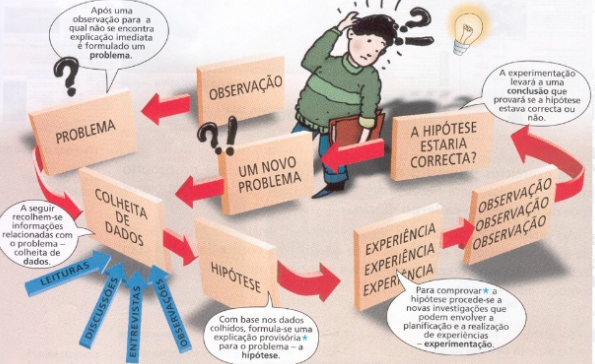
\includegraphics[scale=0.70]{metodo.png}
    \caption{Fases de uma pesquisa}
    \label{metodo_cient}
\end{figure}

Uma lista completa das normas
observadas pelo \abnTeX\ é apresentada em \citeonline{abntex2classe}.



Este documento deve ser utilizado como complemento dos manuais do \abnTeX\ 
\cite{abntex2classe,abntex2cite,abntex2cite-alf}. Consulte \citeonline{abntex2modelo} para obter
exemplos e informações adicionais de uso de \abnTeX\ e de \LaTeX.






% ----------------------------------------------------------
% Elementos Textuais
% ----------------------------------------------------------
\chapter{Referencial Teórico}

\index{elementos textuais} O Referencial Teórico é um seção dos elementos textuais. A norma ABNT NBR 15287:2011, p. 5, apresenta a
seguinte orientação quanto aos elementos textuais:

\begin{citacao}
O texto deve ser constituído de uma parte introdutória, na qual devem ser
expostos o tema do projeto, o problema a ser abordado, a(s) hipótese(s),
quando couber(em), bem como o(s) objetivo(s) a ser(em) atingido(s) e a(s)
justificativa(s). É necessário que sejam indicados o referencial teórico que
o embasa, a metodologia a ser utilizada, assim como os recursos e o cronograma
necessários à sua consecução.\citeonline{abntex2classe}
\end{citacao}

Deve-se apresentar a fundamentação teórica que orientará o estudo. Recomenda-se situar a grande área, subárea e objeto de estudo. Se for necessário pode ser feito um resgate histórico para demonstrar a evolução da área. Faz-se necessário relatar o momento vivido pela área (Marco Teórico - Estado da Arte) geralmente intitulado de Trabalhos Relacionados.

O Referencial Teórico é considerado como um elemento de controle de toda a pesquisa, desde a problematização inicial. O pesquisador irá interpretar seu objeto de estudo de acordo com a concepção teórica de uma ou toda a obra de um autor ou de um objeto ou produto ou de um conjunto de autores (esta condução varia de acordo com cada área de conhecimento). Todas as etapas do projeto são definidas conforme esta escolha. Apresenta-se de modo aprofundado, respondendo quais os princípios, categorias, conceitos ou teorias fundamentam a pesquisa. Deve estar de acordo com o tema formulado e o raciocínio desenvolvido nas fases anteriores. 


%===== Seção de Metodologia ==============

\chapter{Metodologia}

\index{elementos textuais} A metodologia em um Projeto de Pesquisa preocupa-se muito mais com a classificação da pesquisa do que propriamente com a condução e execução do trabalho. Porém, o ideal é apresentar o detalhamento metodológico da pesquisa incluindo aspectos técnicos de execução específicos da área. Desta forma, o leitor ou avaliador poderá ter clareza do que será feito e como será feito. Lembrando que a execução metodológica deve estar alinhada com os objetivos específicos descritos na Introdução. 

\begin{enumerate}
\item
Tipo de Pesquisa: Pode-se fazer pesquisa bibliográfica, documental, experimental, estudo de caso e outros tipos. Na área tecnológica, a maioria dos trabalhos é classificada como experimental (quando há um protótipo desenvolvido) e estudo de caso (se situação problemática é relacionada à uma empresa).
\item
	Universo, População e Amostragem:
Deve-se identificar a população da qual você está retirando a sua amostra. Por exemplo, se sua pesquisa envolve os alunos do curso de Sistemas de Informação, sua população é o número total destes alunos, por exemplo 250 alunos. Se você decide então fazer uma amostragem, digamos de 10\%, então sua amostra para fins de sua pesquisa será de 25 alunos.
\item
	Coleta de Dados:
Deve-se indicar como irá operacionalizar a coleta os dados (questionários, check-lists, entrevistas, etc).
\item
	Análise e Interpretação dos Resultados:
Descreve-se neste item como será a análise dos resultados da pesquisa (se a pesquisa for qualitativa, as respostas podem ser interpretadas global ou individualmente, se a pesquisa for  quantitativa, você provavelmente irá utilizar a estatística descritiva ( média, mediana, moda, desvio padrão, tendência central) ou estatística inferencial (regressão linear bivariada, multivariada, etc).
\item
Os gêneros de pesquisa:
Em outra forma descritiva, a pesquisa também pode ser detalhada em termos de métodos obedecendo a classificação de natureza, objetivos, procedimentos, objeto e abordagem:
\begin{enumerate}
\item	Quanto à natureza
\begin{itemize}
\item Teórica - dita como conceitual, procura rever teorias ou formular novas idéias, parâmetros teórico-doutrinários, conceitos.
Metodológica - destina-se a redimensionar novos procedimentos de investigação, modos inovadores de construir ciência, transformação de metodologias tradicionais, introdução de novas técnicas de se conceber o objeto de estudo.
\item Empírica - dedica-se a mensurar a realidade; considera fatores sociais, políticos e econômicos na análise, em outras palavras, parte de constatações empíricas ou da realidade social para solucionar o problema da pesquisa; além disso, formula observações do real e propõe transformações do mesmo enquanto objeto de investigação.
\item Prática - embora semelhante à empírica, difere-se desta por se voltar a intervenções concretas no ambiente político, jurídico, ou sócio-cultural; transformações durante o trajeto da investigação ou análises que proponham novos rumos para a realidade social são os objetivos desse gênero.
\end{itemize}
\item
	Quanto aos objetivos
\begin{itemize}
\item Pesquisa exploratória
- Proporcionar maior familiaridade com o problema;
Levantamento bibliográfico ou entrevistas;
Pesquisa bibliográfica ou estudo de caso.
\item Pesquisa descritiva
- Fatos são observados, registrados, analisados, classificados e interpretados, sem interferência do pesquisador.
- Uso de técnicas padronizadas de coleta de dados (questionário e observação sistemática).
\item Pesquisa explicativa
- Identifica fatores determinantes para a ocorrência dos fenômenos.
- Ciências naturais – método experimental; ciências sociais – método observacional.
\end{itemize}
\item  Quanto aos procedimentos
\begin{itemize}
\item Pesquisa de campo – observação e coleta de dados diretamente no local da ocorrência dos fatos.
\item Pesquisa de fonte documental – pesquisa bibliográfica e documental.
\end{itemize}

\item
	Quanto ao objeto
\begin{itemize}
\item Pesquisa bibliográfica/documental – elaborada a partir de material já publicado (livros de quaisquer espécies, artigos de periódicos).
Pesquisa de laboratório – pesquisador procura refazer as condições de um fenômeno a ser estudado, para observá-lo sob controle.
\item Pesquisa de campo – pesquisador constrói um modelo da realidade, definindo formas de observá-la, formas de acesso a esse campo, os participantes e o campo da pesquisa.
\end{itemize}

\item
	Quanto à forma de abordagem
\begin{itemize}
\item Pesquisa quantitativa – traduz em números as opiniões e informações para serem classificadas e analisadas. Utilizam-se técnicas estatísticas.

\item Pesquisa qualitativa – é descritiva. As informações obtidas não podem ser quantificáveis. Os dados obtidos são analisados indutivamente. A interpretação dos fenômenos e a atribuição de significados são básicas no processo de pesquisa qualitativa. 
\end{itemize}
\end{enumerate}
\end{enumerate}

%===== Seção de Metodologia ==============

\chapter{Cronograma}

\index{elementos textuais}
O cronograma tem por objetivo prever as ações distribuídas de acordo com o tempo previsto de pesquisa. O cronograma deve estar alinhado com os objetivos específicos e com a metodologia. Nos objetivos específicos tem-se “o que vou fazer”, na metodologia, “como vou fazer” e no cronograma, “quando vou fazer”.

A  \autoref{tabela_cronog} apresenta o cronograma de execução da pesquisa. 

\begin{table}[!htb]
\centering
\caption{Cronograma de Atividades}
\label{tabela_cronog}
\begin{tabular}{@{}llll@{}}
\toprule
\textit{Atividades}                  & \textit{Mês}       & \textit{Ano}   \\ \midrule
Revisão Sistemática                  & Julho              & 2016      \\
Análise de Trabalhos Relacionados    & Agosto             & 2016      \\
Construção da Arquitetura            & Setembro           & 2016      \\
Implementação do Sistema             & Outubro            & 2016      \\
Avalição e Testes                    & Fevereiro          & 2017      \\
                                     &                    &           \\ \bottomrule
\end{tabular}
\end{table}




% ----------------------------------------------------------
% Capitulo com exemplos de comandos inseridos de arquivo externo 
% ----------------------------------------------------------

\include{abntex2-modelo-include-comandos}

% ---
% Finaliza a parte no bookmark do PDF
% para que se inicie o bookmark na raiz
% e adiciona espaço de parte no Sumário
% ---
\phantompart



% ----------------------------------------------------------
% ELEMENTOS PÓS-TEXTUAIS
% ----------------------------------------------------------
\postextual

% ----------------------------------------------------------
% Referências bibliográficas
% ----------------------------------------------------------
\bibliography{abntex2-modelo-references}

% ----------------------------------------------------------
% Glossário
% ----------------------------------------------------------
%
% Consulte o manual da classe abntex2 para orientações sobre o glossário.
%
%\glossary

% ----------------------------------------------------------
% Apêndices
% ----------------------------------------------------------

% ---
% Inicia os apêndices
% ---
\begin{apendicesenv}

% Imprime uma página indicando o início dos apêndices
\partapendices

% ----------------------------------------------------------
\chapter{Exemplo de um apêndice A}
% ----------------------------------------------------------



% ----------------------------------------------------------
\chapter{Exemplo de um apêndice B}
% ----------------------------------------------------------


\end{apendicesenv}
% ---


% ----------------------------------------------------------
% Anexos
% ----------------------------------------------------------

% ---
% Inicia os anexos
% ---
\begin{anexosenv}

% Imprime uma página indicando o início dos anexos
\partanexos

% ---
\chapter{Exemplo de um primeiro anexo}
% ---


% ---
\chapter{Exemplo de um segundo anexo}
% ---



% ---
\chapter{Exemplo de um terceiro anexo}
% ---



\end{anexosenv}

%---------------------------------------------------------------------
% INDICE REMISSIVO
%---------------------------------------------------------------------

\phantompart

\printindex


\end{document}
